%%%%%%%%%%%%%%%%%%%%%%%%%%%%%%%%%%%%%%%%%%%%%%%%%%%%%%%%%%%%%%%%%%%%%%%%
%                                                                      %
%     File: Thesis_Background.tex                                      %
%     Tex Master: Thesis.tex                                           %
%                                                                      %
%     Author: Andre C. Marta                                           %
%     Last modified :  2 Jul 2015                                      %
%                                                                      %
%%%%%%%%%%%%%%%%%%%%%%%%%%%%%%%%%%%%%%%%%%%%%%%%%%%%%%%%%%%%%%%%%%%%%%%%



\chapter{Investing and entering the market with a new product}
\label{chapter:1}

%Insert your chapter material here...


%%%%%%%%%%%%%%%%%%%%%%%%%%%%%%%%%%%%%%%%%%%%%%%%%%%%%%%%%%%%%%%%%%%%%%%%
\section{Introduction}
\label{section:overview}

In this chapter we consider a firm that %has no products inserted on the market
is not active in the market and aims to invest in a new product, with an innovation level $\theta$. Therefore, at the investment time, the firm needs to incur an investment cost proportional to the capacity of production $K$. This cost is given by $\delta K$ with $\delta>0$, a sensibility parameter related to the investment\footnote{Check Section \ref{intro:notation} for further details.}. Here we consider that the investment decision is irreversible (meaning that it is not possible to obtain investment costs back) and that the production starts at the same time the investment is undertaken.


The unitary price function $p$ associated to this product is considered to evolve stochastically with the demand process \textbf{X} and it is given by
\begin{equation}
p(X_t)=(\theta-\alpha K) X_t \geq 0
\label{prob1:p}
\end{equation}
where $\alpha>0$ is a sensibility parameter and $X_t$ corresponds to the demand level observed at the instant $t\geq0$. Depending on the authors, $p$ might also be called \textit{demand function}, as it is the case on \cite{rita}, for example. The firm wouldn't fix an unitary negative price to a certain product, since it would imply a negative profit. Therefore $p$ is always positive and hence, it follows that $\theta \geq \alpha K$ must be verified.

The instantaneous profit function $\pi$ is obtained by multiplying the unitary price function $p$ by the quantity wanted to be produced, which, as previously explained, is assumed to be fixed along the production process. Then, it follows that
\begin{equation}
\pi(X_t)=(\theta-\alpha K)K X_t.
\label{prob1:pi}
\end{equation}

\begin{figure}[!htb]
	\centering
	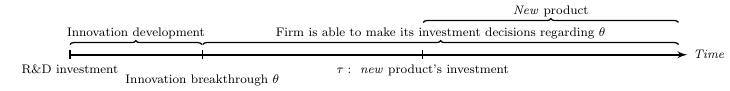
\includegraphics[width=\textwidth]{Prob1_CapOpt/1_timelinet.PNG}
	\caption{Timeline representing the two possible different stages of production and associated decisions. Time is set to start at the innovation breakthrough.}
	\label{1_time}
\end{figure}

Recall that investment timeline is set to start at the precise instant the innovation breakthrough happens, as presented on Figure \ref{1_time}. Only after that instant the firm is able to create the product with an in-putted $\theta$ innovation level.

%%%%%%%%%%%%%%%%%%%%%%%%%%%%%%%%%%%%%%%%%%%%%%%%%%%%%%%%%





%%%%%%%%%%%%%%%%%%%%%%%%%%%%%%%%%%%%%%%%%%%%%%%%%%%%%%%%%

Therefore, when determining the optimal investment time on the new product, we consider as the starting time the instant at which occurs the innovation breakthrough. However when evaluating the value function regarding the complete investment (associated to both R\&D and new product), the starting time corresponds to the time at which the firm decides to invest in R\&D.





%%%%%%%%%%%%%%%%%%%%%%%%%%%%%%%%%%%%%%%%%%%%%%%%%%%%%%%%%%%%%%%%%%%%%%%%


We will address two cases: in the first case, we assume that $K$ is given and, in the second case, we optimize $K$ in order to maximize the profit of the firm. The first case is the easiest to derive and therefore we call it the benchmark model.

%As mentioned before, two models will be derived. The first one corresponds to the benchmark model. The simplest model to be considered. The second one will take into account the maximized instantaneous profit in function of the production capacity $K$. Comparative statics of both models will be made afterwards.


%%%%%%%%%%%%%%%%%%%%%%%%%%%%%%%%%%%%%%%%%%%%%%%%%%%%%%%%%%%%%%%%%%%%%%%%
\section{Stopping Problem}
\label{section:1_theory}



\subsection{Benchmark Model}
\label{subsec:1_bm}

In the benchmark model we want to find when is the optimal investment time such that it leads to the maximization of the expected discounted long-term profit, assuming that this decision is taken in finite time.
%, taking into account all the information previously referred.

%Denoting the time of investment in the new product as $\tau$, our optimization problem can be written as 

%In the benchmark model we want to find when is the optimal time invest in the product (in the sense that maximizes the expected long-term profit), taking into account all the information previously referred.

Denoting the investment time in the new product by $\tau$, our optimization problem can be written as 
\begin{equation}
\sup_\tau \mathds{E}^{X_0=x} \left[ \left( \int_\tau^\infty e^{-rs} \pi(X_s)\ ds - e^{-r \tau} \delta K \right) \ \mathds{1}_{\{\tau<\infty\}} \right]
\label{eq:probz}
\end{equation}
for $\theta, x\in \mathds{R}^+$. Note that $ \mathds{1}_{\{\tau<\infty\}}$ assures that, with probability 1, the decision is made in a finite amount of time.

Putting the discount term in evidence, from \eqref{eq:probz} follows
\begin{equation}
\sup_\tau \mathds{E}^{X_0=x} \left[e^{-r\tau }\left( \int_\tau^\infty e^{-r(s-\tau)} \pi(X_s)\ ds -\delta K \right) \ \mathds{1}_{\{\tau<\infty\}} \right].
\label{probjj}
\end{equation}

We can simplify this expression. Using Tower rule and conditioning on the instant the firm exercises, we obtain that \eqref{probjj} may be written as
\begin{equation}
\sup_\tau \mathds{E}^{X_0=x}\left[ e^{- r\tau} \left( \mathds{E}^{\tau}\left[  \int_\tau^\infty e^{-r(s-\tau) }\pi(X_s)\ ds  \right] -\delta K\right) \mathds{1}_{\{\tau<\infty\}} \right].
\label{eq:probm}
\end{equation}

Focusing on the inner expected value $\mathds{E}^{\tau}\left[  \int_t^\infty e^{-(\tau-s) }\pi(X_s) \ ds  \right]$ and changing its integration variable follows
\begin{equation}
\mathds{E}^{\tau}\left[  \int_0^\infty e^{-rv }\pi(X_{v+\tau})\ dv  \right].
\label{eq:e1}
\end{equation}

%Considering $r-\mu>0$, we have that $ \int_0^\infty \int_\Omega    |e^{-rv }\pi(X_{v+\tau})| \ \mathds{P}(d \omega) \ dv < \infty$. Since $e^{-rv }\pi(X_{v+\tau})$ is a continuous function it follows that is also a measurable function. By both conditions we obtain that it is $[0,\infty) \times \Omega$-integrable. Therefore by Fubini's Theorem we can interchange the integrals, from which follows by \eqref{eq:e1}, that
As we assume that $r-\mu>0$ and $e^{-rv }\pi(X_{v+\tau})$ is a measurable function, by Fubini's Theorem we may interchange the order of integration of \eqref{eq:e1}, obtaining
\begin{equation}
\int_0^\infty\mathds{E}^{\tau}\left[   e^{-rv }\pi(X_{v+\tau}) \right]\ dv
= (\theta-\alpha K)K \int_0^\infty\mathds{E}^{\tau}\left[   e^{-rv } X_{v+\tau} \right]\ dv,
\label{eq:e2}
\end{equation}
where we took into account the expression of the profit function $\pi$.


Let's now focus on the expected value $\mathds{E}^{\tau}\left[   e^{-rv }  X_{v+\tau} \right]$.
Using the fact that the process \textbf{X} is a GBM, it follows that
\begin{align}
\mathds{E}^{\tau}\left[   e^{-rv } X_{v+\tau} \right] 
&= \mathds{E}^{\tau}\left[   X_\tau e^{\left(\mu- \frac{\sigma^2}{2}-r \right) (\tau+v-\tau) + \sigma (W_{\tau+v}-W_\tau)}\right] \nonumber \\
&=X_\tau e^{\left(\mu- \frac{\sigma^2}{2}-r \right) v} \ \mathds{E}^{\tau}\left[ e^{\sigma W_v} \right] \nonumber \\
&=X_\tau e^{\left(\mu- \frac{\sigma^2}{2}-r \right) v} e^{ \frac{\sigma^2}{2} v} \nonumber \\
&=X_\tau e^{(\mu-r)v}.
\label{eq:e4}
\end{align}


In the first step we use the expression associated to the GBM and the fact that, by knowing the investment time $\tau$, we also know the demand level at that time, here represented as $X_\tau$. In the second step, the fact that the Brownian Motion has stationary increments implies that $W_{\tau+v}-W_\tau \overset{d}{=}  W_v$
%, where $W_0=0$ holds since we assumed \textbf{W} to be a standard Brownian Motion.
In the third step we use the fact that $ W_v \sim \mathcal{N}(0,v)$ and the expression for the moment generating function associated to the Normal distribution, from which follows $\mathds{E}\left[e^{sW_v}\right]=e^{\frac{1}{2} s v^2}$. Simplifying the expression we obtain \eqref{eq:e4}.

Plugging the resultant expression \eqref{eq:e4} in \eqref{eq:e2} and solving the integral, we obtain the formula of the terminal cost function associated to this problem - corresponding to the expression between brackets in \eqref{probjj} and \eqref{eq:probm}. We will denote it by $h$ and its expression corresponds to
\begin{equation}
h(x)=\frac{(\theta-\alpha K)K x}{r-\mu}- \delta K.
\label{prob1:h}
\end{equation}
The terminal cost function $h$ represents the discounted long-term cash-flow by acquiring a product when the demand level is $x$. It already includes the investment cost of such decision, given by $\delta K$.
 
Denoting $F$ as the value function associated to this problem, we obtain that our optimization problem, as described in \eqref{eq:probz}, can be written as a standard optimal stopping problem with null running cost function, given by
\begin{equation}
F(x)=\sup_\tau \mathds{E}^{X_0=x}\left[e^{-r\tau } h(X_\tau) \mathds{1}_{\{\tau<\infty\}} \right]=\sup_\tau \mathds{E}^{X_0=x}\left[e^{-r\tau } \left( \frac{(\theta-\alpha K)K X_\tau}{r-\mu}-\delta K \right) \mathds{1}_{\{\tau<\infty\}} \right].
\label{eq:prob3}
\end{equation}


Then, invoking results presented on Chapter \ref{chapter:bc}, in particular \eqref{sol}, it follows that $F$ is defined differently for the continuation and stopping regions, as follows:
%% Recurring to Bellman principle, we have that the solution $F$ verifies the variational inequality given by Hamilton-Jacobi-Bellman (HJB) variational inequality \eqref{HJB} and hence, it is given by

\begin{equation}
F(x)=\begin{cases} a x^{d_1}  \ &, \ x \in \mathcal{C} \\
h(x) \ &, \ x \in \mathcal{S}
\end{cases},
\label{1_F}
\end{equation}
with $d_1$ being the positive root of the polynomial described in \eqref{d1d2}.

As motivated before, we propose that $\mathcal{C}=\{x\in \mathds{R}:x< x_B^* \}$, where $x_B^*$ denotes the demand that triggers the (optimal) decision to invest. Thus we find $a$ and $x_B^*$ using value matching \eqref{valuematch} and smooth pasting \eqref{smoothpasting} conditions, expressed by the corresponding system

%%where coefficient $a$ and the threshold value $x^*$, that defines the boundary between continuation and stopping regions, are found by value matching \eqref{valuematch} and smooth pasting \eqref{smoothpasting} conditions, expressed by the corresponding system
\begin{equation}
\begin{cases} a(x_B^*)^{d_1}=\frac{K(\theta-\alpha K) x^*}{r-\mu} - \delta K \\
ad_1(x_B^*)^{d_1-1}=\frac{K(\theta-\alpha K)}{r-\mu}
\end{cases}
\hspace{5mm} \Rightarrow \ \hspace{5mm}
\begin{cases}
a= \left( \frac{K(\theta-\alpha K) x_B^*}{r-\mu} - \delta K \right)(x_B^*)^{-d_1} = \frac{\delta K (x^*)^{-d_1}}{d_1-1}\\
x_B^*=\frac{d_1}{d_1-1} \frac{ \delta (r-\mu)}{\theta-\alpha K}
\end{cases}
\label{eq:sistema}
\end{equation}


Finally, we obtain that the stopping region associated to this problem is defined as $\mathcal{S}=\{x\in \mathds{R}:x \geq x_B^* \}$ and the optimal stopping time as in \eqref{stoptime}.

%%%%%%%%%%%%%%%%%%%%%%%%%%%%%%%%%%%%%%%%%%%%%%%%%%%%%%%%%%%%%%%%%%%%%%%%%%%%%%%%%%%%


\subsection{Capacity Optimization Model}
\label{subsec:1_com}

Now we consider a more realistic case, in which the firm wants to take the best of its investment by choosing an appropriate capacity of production. This can be achieved by requiring that the capacity of production leads to the maximization of the discounted long-term cash-flow. Therefore our goal is now to find when is the optimal (finite) time to invest and which is the optimal capacity associated to it. This can be stated as
\begin{equation}
\sup_\tau \mathds{E}^{X_0=x} \left[ \max_K \left\{ e^{-r\tau }  \left( \int_\tau^\infty e^{-r(\tau-s)} \pi(X_s)\ ds -\delta K \right) \right\} \mathds{1}_{\{\tau<\infty\}} \right].
\label{eq:probj}
\end{equation}

Manipulating the expression as previously done, we obtain that \eqref{eq:probj} may be written as
\begin{equation}
\sup_\tau \mathds{E}^{X_0=x} \left[ e^{-r\tau } \max_K \left\{ h(X_\tau,K) \right\} \mathds{1}_{\{\tau<\infty\}} \right],
\label{eq:q1}
\end{equation}
with $h$ corresponding to the terminal function deduced in \eqref{prob1:h}, in which we now highlight not only the dependence on the demand level, but also on the capacity of production $K$ chosen at the investment time.

In this section, the capacity optimization model is obtained in two steps, as similarly done in \cite{huis:cap}, for example. In the first step, we calculate the capacity level that optimizes the terminal cost function $h$, which we will denote by $K^*$. In the second, we solve the optimal stopping problem given by $\underset{\tau}{\sup}\ \mathds{E}^{X_0=x}\left[e^{-r\tau}h(X_\tau,K^*) \mathds{1}_{\{\tau<\infty\}} \right]$, in which we are already considering the optimized terminal function (with respect to $K$).

The optimal capacity level $K^*$ is found by analysing the behaviour - namely stationary points and concavity  - of the terminal function $h$, while considering a fix level of demand.

Stationary points are found by calculating the roots of the first partial derivative, which is given by
\begin{equation}
\frac{\partial h }{\partial K}(x,K)=  \frac{(\theta-2\alpha K)x}{r-\mu} - \delta,
\label{1_dK}
\end{equation}
following  that $h$ has a unique stationary point corresponding to
$K=\frac{\theta}{2\alpha}-\frac{\delta (r-\mu)}{2 \alpha x}$.


Analysing its second partial derivative of $h$, we obtain that
\begin{equation}
\frac{\partial^2 h }{\partial K^2}(x,K)=  -\frac{2\alpha x}{r-\mu},
\label{1_d2K}
\end{equation}
which is negative, since the every state of the GBM is positive, $\alpha>0$ and $r-\mu>0$ . Therefore, $h$ is a concave function and 
%the capacity value found before corresponds to 
thus the zero of the first derivative is its global maximizer. Denoting it by $K^*$, we have that
\begin{equation}
K^*:= \arg \max_K h(x,K)=\frac{\theta}{2\alpha}-\frac{\delta (r-\mu)}{2 \alpha x},\ \forall x 
\label{eq:K41}
\end{equation}

Since the firm can only produce a positive quantity, we need to verify $K^* >0 $ which is equivalent to the condition  $x > \frac{\delta(r-\mu)}{\theta} $ for any considered demand level $x \in \mathds{R}^+$, which holds, in view of our assumptions on $\delta, \ r, \ \mu$ and $\sigma$.
%Observe that $K^*$ grows with the demand level and grows linearly with the innovation level (meaning that the higher the demand or technology level is, the larger is the optimal quantity that should be produced).

Now we proceed to the second step. Evaluating $h$ at its optimal capacity level $K^*$ we obtain
$$h(x,K^*)=\frac{(\theta x -\delta (r-\mu))^2}{4 \alpha (r-\mu) x}.$$

Denoting $F^*$ as the value function associated to the optimal stopping problem in \eqref{eq:41}, the optimization problem can be stated as
\begin{equation}
F^*(x)=\sup_\tau \mathds{E}^{X_0=x}\left[ e^{-r\tau}h(X_\tau,K^*) \mathds{1}_{\{\tau<\infty\}} \right]
= \sup_\tau \mathds{E}^{X_0=x}\left[ e^{-r\tau} \frac{(\theta X_\tau -\delta (r-\mu))^2}{4 \alpha (r-\mu) X_\tau} \mathds{1}_{\{\tau<\infty\}}\right],
\label{eq:41}
\end{equation}
which is again a standard optimal stopping problem with null running cost function. Similarly to the benchmark model, we obtain that the value function associated to \eqref{eq:41} satisfies the HJB variational inequality \eqref{HJB}. Therefore $F^*$ is such that
\begin{equation}
F^*(x)=\begin{cases} b x^{d_1}  \ &, \ x \in \mathcal{C} \\
h(x,K^*) \ &, \ x \in \mathcal{S}
\end{cases},
\label{1_F*}
\end{equation}
with $\mathcal{C}=\{x\in \mathds{R}:x< x_C^* \}$ the continuation region, where $x_C^*$ stands for the demand level that triggers the optimal investment.

Then, coefficient $b$ and the threshold value $x_C^*$ are found by value matching \eqref{valuematch} and smooth pasting conditions \eqref{smoothpasting}, expressed by the corresponding system
\begin{equation}
\begin{cases} b (x_C^*)^{d_1}=\frac{(\theta x -\delta (r-\mu))^2}{4 \alpha (r-\mu) x} \\
b d_1(x_C^*)^{d_1-1}=\frac{\theta^2 (x_C^*)^2 -\delta^2 (r-\mu)^2}{4 \alpha (r-\mu) (x_C^*)^2}
\end{cases}.
\label{eq:sistema3}
\end{equation}

We get two possible positive roots for the threshold level: $x^*_{C,1}=\frac{d_1+1}{d_1-1} \frac{ \delta (r-\mu)}{\theta-\alpha K}$ and $x^*_{C,2}=\frac{\delta  (r-\mu )}{\theta }$. However, after some manipulation, we exclude the second one $x^*_{C,2}$, since the coefficient $b$ associated to it takes a null value. This is an absurd, since it would lead to a null value function for any demand level smaller than $x^*_{C,2}$, neglecting potential investment decisions in the future.
%possibility of investing in the future is also valuable.
Therefore we obtain that the threshold level and coefficient $b$ in \eqref{eq:sistema} are given, respectively, by
\begin{align}
 &x_C^*=\frac{d_1+1}{d_1-1} \frac{ \delta (r-\mu)}{\theta} \label{eq:prob1_xC}\\
 &b=\left( \frac{(\theta x -\delta (r-\mu))^2}{4 \alpha (r-\mu) x_C^*} \right)(x_C^*)^{-d_1} = \frac{\delta \theta}{\alpha (d_1^2-1)} \left( \frac{d_1+1}{d_1-1} \frac{ \delta (r-\mu)}{\theta} \right)^{-d_1} \nonumber
\end{align}
Finally the stopping region coincides with $\mathcal{S}=\{x\in \mathds{R}:x< x_C^* \}$ and the optimal stopping time as in \eqref{stoptime}.

Now we analyse the optimal capacity level $K^*_C$. If at the innovation breakthrough - that we set to be the initial instant when deducting the optimal investment times - we have $X_0<x^*_C$, then the investment decision will happen at the same instant the demand reaches level $x^*_C$. 
%, by paying $\delta K^*_C$. 
As done in \cite{huis:cap}, the optimal capacity level is obtained by evaluating $K^*$, as defined in \eqref{eq:K41}, at the threshold demand level $x^*_C$ \eqref{eq:prob1_xC}, leading to
\begin{equation}
K^*_C=\frac{2 \sigma ^2 \theta}{\alpha \left(\sigma ^2 \left(\sqrt{\frac{4 \mu ^2}{\sigma ^4}-\frac{4 \mu }{\sigma ^2}+\frac{8 r}{\sigma ^2}+1}+3\right)-2 \mu \right)}.
\label{prob1:K*}
\end{equation}

%Since the demand process is continuous, this is the only optimal capacity level able to be verified, on this situation.
% when we have a smaller demand than the threshold at the instant the innovation breakthrough happens.
%Note that since the demand process is continuous, there is no possibility on investing $K^*(x_t), \ x_t>x_C^*, \ t>0$, since we assume the investment to be at the precise instant that $x^*_C$ is observed.

However it might be the case that when the breakthrough happens, we observe an equal or higher demand than the threshold $x^*_C$. This one is not as interesting as the previously mentioned. The firm will invest at the same instant the breakthrough happens choosing an optimal capacity given by evaluating $K^*$, as defined in \eqref{eq:K41}, at the observed demand level at the breakthrough. This case won't be addressed on Comparative Statics (Section \ref{prob1:cs}).



%%%%%%%%%%%%%%%%%%%%%%%%%%%%%%%%%%%%%%%%%%%%%%%%%%%%%%%%%%%%%%%%%%%%%%%%%%%%%%%%%%%


\section{Comparative Statics}
\label{prob1:cs}

In this section we study the behaviour of the decision threshold $x^*_B$ \eqref{eq:sistema} and $x^*_{C}$ \eqref{eq:prob1_xC} and $K^*$ as described in \eqref{prob1:K*}, with
the different parameters. Comparisons between the benchmark and capacity optimization models will be also be presented.

\subsection{Benchmark Model}

%\textbf{Proposition:}
\begin{prop}
	\label{1_prop1}
The decision threshold $x^*_B$ increases with $r, \sigma, \ K, \ \alpha$ and  $\delta$, and decreases with $\theta$ and $\mu$.
\end{prop}

\textbf{Proof:}

%Before showing the results stated, we focus on $\phi$ since it will be a recurrent expression in most comparative statics sections. This is given by
As it will play an important role, we start by defining the following quantity:
\begin{equation}
\phi:=\sqrt{\frac{4 \mu ^2}{\sigma ^4}-\frac{4 \mu }{\sigma ^2}+\frac{8 r}{\sigma ^2}+1}.
\label{phi}
\end{equation}

With simple calculus and in view of the admissible values for $\mu, \ \sigma$ and $r$, we obtain that the value inside the square root is always positive and hence $\phi$ is well defined and non-negative.
%We analyse the expression inside the square root in order to infere about $\phi$ %as well as some extra constraints regarding our problem. However, since that expression only has imaginary roots regarding parameter $\mu$ or roots that are not allowed our problem constraints regarding parameters $r$ and $\sigma$ it follows that it is always positive, so it $\phi>0, \ \forall r, \mu, \sigma$ in our problem domains.	

Now we are in position to explain the stated results.

Regarding $r$, we obtain
$$\frac{\partial x^*_B}{\partial r}=\frac{\delta  \left(-(d_1-1) d_1 \sigma ^2 \phi-2 \mu +2 r \right)}{(d_1-1)^2 \sigma ^2 (\alpha  K-\theta ) \sqrt{\frac{4 \mu ^2}{\sigma ^4}-\phi}}>0,$$
Given the constraints of our problem, its denominator is well-defined and negative so as its numerator\footnote{Numerator's roots are given by $\mu \in \left\{r, \frac{1}{2}\left(\sigma ^2\pm\sqrt{\sigma ^4-8 r \sigma ^2}\right) \right\}$ and $\sigma = \pm i \frac{ \mu  (\mu -r)}{\sqrt{-\mu ^3+2 r^3-5 \mu  r^2+4 \mu ^2 r}}$.
%	Regarding the first case we have that only admissible root w.r.t. $\mu$ is given by $r$:	
%	the second pair of roots is admissible \textit{iff} $\sqrt{\sigma^4-8r \sigma^2}$ is well-defined \textit{iff} $\sigma^4-8r \sigma^2>0$ iff $r<-6 \sigma^2$, which is an absurd since we are considering positive interest rates.

%	 Note that,\\
%$\forall r, \ \sigma \in (0,1) \ \Rightarrow \ \sigma ^4-8 r \sigma ^2<0 \ \Rightarrow \ \frac{1}{2}\left(\sigma ^2\pm\sqrt{\sigma ^4-8 r \sigma ^2}\right \} \notin \mathds{R}.$ 

Regarding the roots in terms of $\mu$ we observe that none of them are admissible in our domain. The first one ($r=\mu$) is excluded since we consider $r>\mu$. The second pair $\left(\mu=\frac{1}{2}\left(\sigma ^2\pm\sqrt{\sigma ^4-8 r \sigma ^2}\right) \right)$ is also excluded: 
\begin{align*}
\frac{1}{2}\left(\sigma ^2-\sqrt{\sigma ^4-8 r \sigma ^2}\right)>r & \ \Leftrightarrow \  (\sigma ^2-2r)^2= \sigma^4-4\sigma^2 r +4 r^2 > -8 r \sigma^2+\sigma^4\\
&\overset{r>0}{\Leftrightarrow} \sigma^2+r>0, \qquad \forall r, \sigma>0 \ \forall \mu<r
\end{align*}
is always verified and $\frac{1}{2}\left(\sigma ^2+\sqrt{\sigma ^4-8 r \sigma ^2}\right)>\frac{1}{2}\left(\sigma ^2-\sqrt{\sigma ^4-8 r \sigma ^2}\right)>r$, resulting that none of them are valid.

Since no imaginary roots are possible regarding our context, none of the two possible roots for $\sigma$ is admissible in our problem. Hence, it follows that the numerator never changes its sign. Evaluating for any value of $\mu, \ \sigma$ and $r$ we obtain that $-(d_1-1) d_1 \sigma ^2 \phi-2 \mu +2 r <0$, showing this way that the numerator is negative. },
from which the result follows.

%Thus since the expression on the numerator is continuous in each of its parameters and takes a positive value when testing for given values, it follows that it is always positive with respect to our problem domain.

Regarding $\sigma$, we obtain
\begin{equation}
\frac{\partial x^*_B}{\partial \sigma}=\frac{2 \delta  (r-\mu) \left(-2 \mu ^2+\mu  \sigma ^2 \left(\phi+1\right)-2 r \sigma ^2\right)}{(d_1-1)^2 \sigma ^5 (\alpha  K-\theta ) \phi}>0
\label{1_xBs}
\end{equation}
Again, given the constraints of our problem, the denominator is negative.
Since $r-\mu>0$ and $-2 \mu ^2+\mu  \sigma ^2 \left(\phi+1\right)-2 r \sigma ^2<0$
\footnote{We obtain that the roots of the polynomial $-2 \mu ^2+\mu  \sigma ^2 \left(\phi+1\right)-2 r \sigma ^2$ correspond to $r \in \{0, \ \mu \}$ and both are impossible in the domain of our problem. Then evaluating for any value of $\mu, \ \sigma$ and $r$ we obtain the result stated.}, the denominator is also negative, from which the result follows.

% the numerator, we found that it has no possible roots on problem domain. Thus, since $-2 \delta  (\mu -r) \left(-2 \mu ^2+\mu  \sigma ^2 \left(\phi+1\right)-2 r \sigma ^2\right) |_{\mu=0}<0$ and the numerator is continuous with respect to each of its parameters, it follows that it is negative.



Regarding $K$, $\alpha$, $\delta$ and $\mu$, we  immediately obtain
\begin{align*}
\frac{\partial x^*_B}{\partial K}&=\frac{\alpha  \delta  d_1 (r-\mu )}{(d_1-1) (\theta -\alpha  K)^2}>0\\
\frac{\partial x^*_B}{\partial \alpha}&=\frac{\delta  d_1 K (r-\mu )}{(d_1-1) (\theta -\alpha K)^2}>0\\
\frac{\partial x^*_B}{\partial \delta}&=\frac{d_1 (r-\mu )}{(d_1-1) (\theta -\alpha  K)}>0\\
\frac{\partial x^*_B}{\partial \theta}&=-\frac{\delta  d_1 (r-\mu )}{(d_1-1) (\theta -\alpha  K)^2}<0.
\end{align*}

%Regarding $\delta$, we obtain
%$$\frac{\partial x^*_B}{\partial \delta}=\frac{d_1dd1} (r-\mu )}{(d_1dd1}-1) (\theta -\alpha  k)}>0.$$

Regarding $\mu$, we obtain
$$\frac{\partial x^*_B}{\partial \mu}= \frac{   \delta \left( (d_1-1) d_1 \sigma ^4 \phi -2 \mu ^2+\mu  \sigma ^2 \phi+1 \right)+r \left(2 \mu -\sigma ^2 \left(\phi+1\right)\right)}{(d_1-1)^2 \sigma ^4 (\alpha K-\theta ) \phi}<0.$$
It is possible to conclude that the denominator is negative. On the other side, the numerator is positive\footnote{We obtain the same pair of non-admissible roots as stated in the above footnote. Then evaluating for any value of $\mu, \ \sigma$ and $r$ we obtain the result stated.}, from which the result follows. %taking into account the domain of our problem, we obtain that there are no possible roots for the numerator. 
%Thus since the expression in the numerator is continuous in each of its parameters and takes a positive value when testing for given possible values, it follows that it is always positive with respect to our domain.
 
 
\begin{flushright}
 $\square$
\end{flushright}


\subsection{Capacity Optimization Model}

\begin{prop}
	\label{1_prop2}
The decision threshold $x^*_C$ increases with $r, \ \sigma$ and $\delta$, decreases with $\theta$ and has a non-monotonic behaviour with  $\mu$. None of any other parameters have effect on $x^*_C$.
\end{prop}

\textbf{Proof:}

Recall the expression of $x^*_C$ given in \eqref{eq:prob1_xC}. One can immediately notice that it is not dependent on parameters $\alpha$ and $K$. Therefore we proceed with the analysis of $x^*_C$ with respect to the other parameters.

Regarding $r$, we obtain
$$\frac{\partial x^*_C}{\partial r}=\frac{\delta  \left(\left(d_1^2-1\right) \sigma ^2  \phi+4 \mu -4 r\right)}{(d_1-1)^2 \theta  \sigma ^2 \phi}>0.$$
Taking into account our problem constraints and after manipulating the expression, we obtain that both denominator and numerator are positive, from which the result holds.
% he denominator above is positive and, after simple calculus . The numerator is a continuous function with respect to its parameters and has no roots in the domain of our problem. Thus, after testing for given possible values, it follows that it is always positive with respect to our domain.


Regarding $\sigma$, we obtain
$$\frac{\partial x^*_C}{\partial \sigma}=\frac{4 \delta  (\mu -r) \left(-2 \mu ^2+\mu  \sigma ^2 (1+\phi)-2 r \sigma ^2\right)}{(d_1-1)^2 \theta  \sigma ^5 \phi}>0.$$
From the negativity of the numerator in  \eqref{1_xBs}, it follows that the numerator of above expression is also positive. Since the denominator is also positive, the result holds.
%Note that its denominator is positive.
%Analyzing the numerator, we found that it has no possible roots on the domain of our problem. Thus since the expression in the numerator is continuous in each of its parameters and takes a positive value when testing for given possible values, it follows that it is always positive with respect to our domain.

Regarding $\delta$, $\theta$ and $\mu$, we immediately obtain 
\begin{align*}
\frac{\partial x^*_C}{\partial \delta}&=\frac{(d_1+1) (r-\mu )}{(d_1-1) \theta }>0,\\
\frac{\partial x^*_C}{\partial \theta}&=-\frac{\delta  (d_1+1) (r-\mu )}{(d_1-1) \theta^2}<0\\
\frac{\partial x^*_C}{\partial \mu}&=\frac{\delta}{(d_1-1)^2 \theta} \left( 1-d_1^2 +(r-\mu)\left(-1+\frac{2\mu-\sigma^2}{\phi \sigma^2} \right) \right)= \begin{cases}
<0 \quad \text{for} \ \mu<\frac{\sigma^2}{2}\\
>0 \quad \text{for} \ \mu>\frac{\sigma^2}{2}
\end{cases}.
\end{align*}

%Regarding $\mu$, we obtain
%$$\frac{\partial x^*_C}{\partial \mu}=\frac{\delta}{(d_1-1)^2 \theta} \left( 1-d_1^2 +(r-\mu)\left(-1+\frac{2\mu-\sigma^2}{\phi \sigma^2} \right) \right)= \begin{cases}
%<0 \quad \text{for} \ \mu<\frac{\sigma^2}{2}\\
%>0 \quad \text{for} \ \mu>\frac{\sigma^2}{2}
%\end{cases}.$$
\begin{flushright}
 $\square$
\end{flushright}


\subsubsection{Numerical comparisons between the Benchmark and the Capacity Optimization Models}

%To illustrate results above mentioned we performed some numerical illustrations, using software \textit{Mathematica} and its function \texttt{Manipulate}. However here we are only able to present static plots - we leave to the interested ones, to check the results achieved with \texttt{Manipulate}.

%Unless it is written the opposite, the following parameter values were considered:

Given the expressions for $x^*_B$ and $x^*_C$, it follows that
$$ \frac{x^*_B}{x^*_C}=\frac{d_1}{d_1-\alpha K} \frac{\theta}{\theta-\alpha K},$$
from where we conclude that $x^*_B$ may be smaller or larger than $x^*_C$, depending, in particular, on how large is $K$. Thus we resort to a numerical illustration, assigning values to the involved parameters.

We use the following values, unless stated otherwise:
%One relevant question in terms of the investment decision is to assess whether the optimization capacity leads to postpone or not the investment thresholds for both models, using numerical illustrations. We use, for this objective, the software \texttt{Mathematica} and, unless stated otherwise, the following values:

\begin{table*}[!htb]
	\centering
	\begin{tabular}{lllllll}
		 $\bullet$ & $\mu=0.03$     &  & \hspace{7cm} &  &  $\bullet$ & $\alpha=0.01$ \\
		 $\bullet$ & $\sigma=0.005$ &  & \hspace{7cm} &  &  $\bullet$ & $\theta=10$   \\
		 $\bullet$ & $r=0.05$       &  & \hspace{7cm} &  &  $\bullet$ & $K=100$       \\
		 $\bullet$ & $\delta=2$                                
	\end{tabular}
%\caption{bjde}
\end{table*}	
%\begin{itemize}
%		\item $\mu=0.03$
%		\item $\sigma=0.005$ 
%		\item $r=0.05$
%		\item $\delta=2$
%		\item $\alpha=0.01$
%		\item $\theta=10$
%		\item $K=100$	
%\end{itemize}

\begin{figure}[!htb]
	\begin{subfigmatrix}{2}
		\subfigure[Behaviour of the threshold value with respect to the benchmark model (blue) and the capacity optimized model (orange), considering capacity levels $K \in [0, \theta/\alpha=1000)$ and the value that $x^*_B$ takes when considering $K^*_C \simeq 375$ (black dot).]{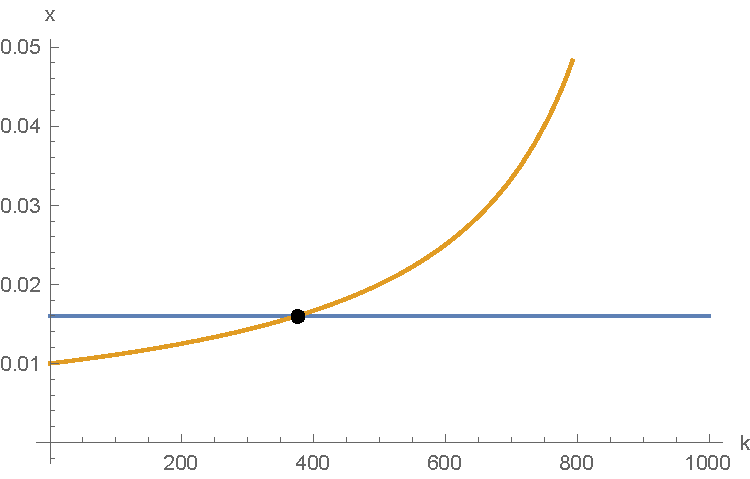
\includegraphics[width=0.45\textwidth]{Prob1_CapOpt/xopt_k.pdf}}
		\subfigure[Evaluation of value functions $F$, considering capacity equal to 200 (darkest blue), $K=K^*_C \simeq 375$ (mid-blue) and 600 (lighest blue), and $F^*$ (orange) with respective demand threshold values presented (black w.r.t. Benchmark Model and grey w.r.t. Capacity Optimization Model)]{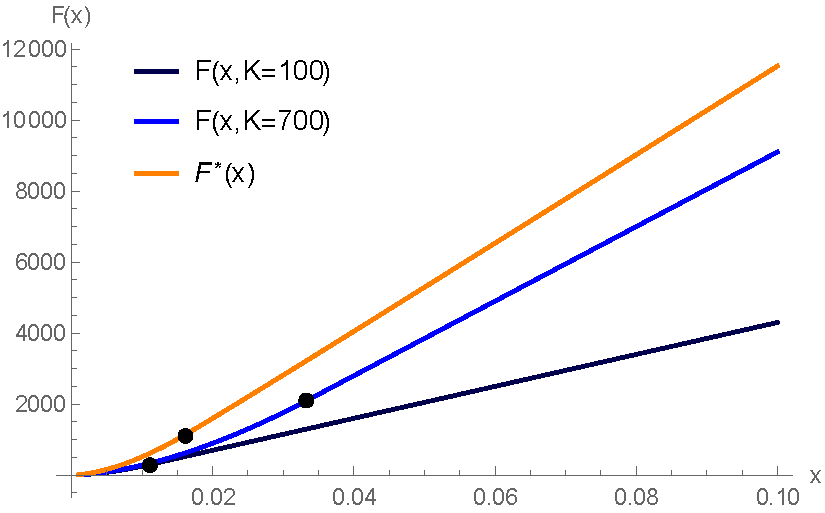
\includegraphics[width=0.45\textwidth]{Prob1_CapOpt/F_k100700.pdf}}
	\end{subfigmatrix}
	\caption{Influence of the chosen capacity $K$ in the threshold values $x^*_B$ and $x^*_C$ and respective value functions $F$ and $F^*$.}
	\label{fig:Kvar}
\end{figure}

We start by illustrating how $x^*_B$ and $x^*_C$ are related by the capacity level $K$. On Figure \ref{fig:Kvar} (a), the behaviour of $x_B^*$ w.r.t the capacity chosen.
% one verifies (as expected) that only $x_B^*$ is influenced by the capacity chosen. A similar behaviour is verified for $\alpha$ since $x^*_B$ depends on both parameters the same way.

Although the threshold $x_B^*$ may be smaller, greater or equal to $x^*_C$ (depending on the capacity $K$ chosen), we always verify that $F^*(x) \geq F(x,K), \ \forall x, K$ considered in the domain of our problem. Figure \ref{fig:Kvar} confirms this precise fact. Its most intriguing case is $F(x,K^*_C)$, which has the same threshold level as the optimal capacity level and verifies: $F^*(x)=F(x,K^*_C), \ \forall x \leq x^*_C$, however 
%for demand values greater than $x_C^*$ we obtain 
$F^*(x)>F(x,K^*_C), \ \forall x > x^*_C$. This is justified by the fact that $F(x,K^*_C)$ considers solely capacity $K_C^*$\footnote{Recall by \eqref{prob1:K*} that $K^*_C$ corresponds to the optimal capacity $K^*$, as described in \eqref{eq:K41}, evaluated at $x_C^*$}, which doesn't maximize the terminal function for demand levels greater than $x_C^*$, while $F^*(x)$ considers the optimal capacity associated to each level of demand, leading to a greater value function.

%, as can be seen on the rightmost side of Figure \ref{fig:Kvar}. Here we have represented value functions $F(x,K)$ defined as in \eqref{1_F}, with the dependence on the capacity $K$ highlighted, and $F^*$ is as defined in \eqref{1_F*}. 



\begin{figure}[!htb]
	\begin{subfigmatrix}{3}
		\subfigure[$r \in ( \mu, 1)$]{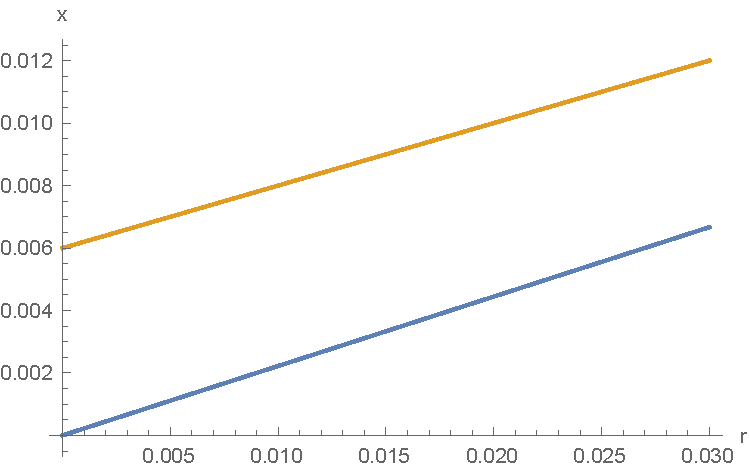
\includegraphics[width=0.32\textwidth]{Prob1_CapOpt/xopt_r.pdf}}
		\subfigure[$\sigma \in (0.0001,1)$]{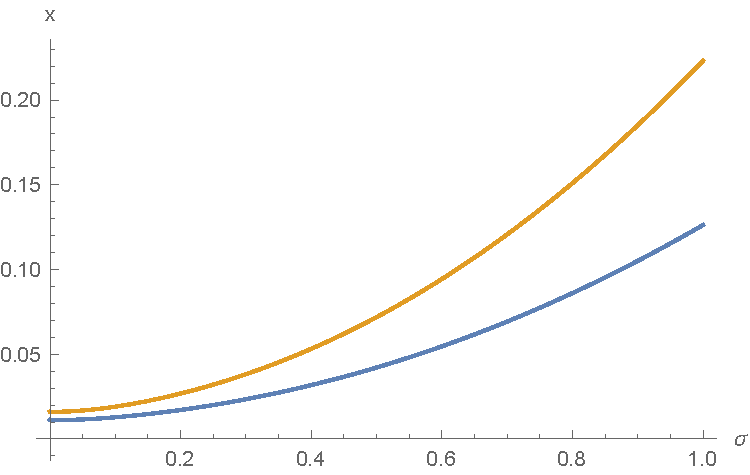
\includegraphics[width=0.32\textwidth]{Prob1_CapOpt/xopt_sigma.pdf}}
		\subfigure[$\delta \in (0,10)$]{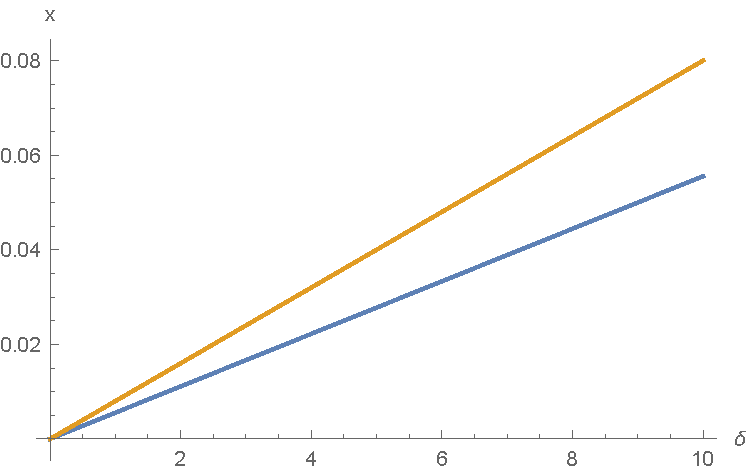
\includegraphics[width=0.32\textwidth]{Prob1_CapOpt/xopt_delta.pdf}}
	\end{subfigmatrix}
	\caption{Behaviour of the threshold value with respect to the benchmark model (blue) and the capacity optimized model (orange) as a function of increasing parameters $r$ (a), $\sigma$ (b)  and $\delta$ (c).}
	\label{fig:sigm}
\end{figure}
On Figure \ref{fig:sigm} (a) we observe that in both situations the decision is postponed with increasing interest rate. This is explainable as: the larger the $r$, the larger is the expected discounted cash-flow and therefore we need to observe larger values of the demand to balance the money lost due to runway devaluation and future earnings.
%we observe that the greater the discount rate $r$ is, the greater the currency devaluation is, when evaluating the expected cash-flow to be earned. Thus, in order to justify the irreversible investment that the firm needs to incur on the new product, we need to observe large values of demand to balance the money lost due to currency devaluation and the future earnings.

Figure \ref{fig:sigm} (b) shows that both thresholds increase with volatility. This in accordance with references \cite{hagspiel:cap} and \cite{rita}, for instance. In fact this is an expected result from real options: by increasing the volatility, the investment is postponed.
% which works describe that when uncertainty is high, there is a delay time to invest, which is here reflected on an higher demand level.

Figure \ref{fig:sigm} (c)shaows that the greater the sensibility parameter $\delta$ is, the larger are the investment sunk cost, leading to a delay on the investment, in the sense that it will only be made if high demand values are observed.

\begin{figure}[!htb]
	\begin{subfigmatrix}{2}
		\subfigure[$\sigma=0.05$]{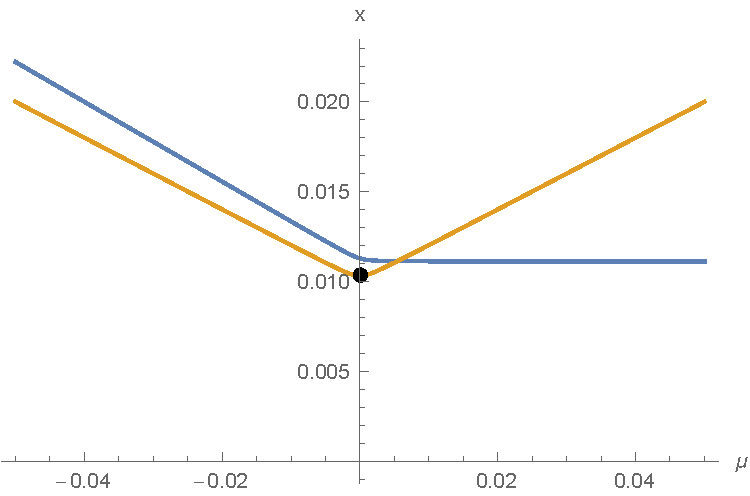
\includegraphics[width=0.45\textwidth]{Prob1_CapOpt/xopt_mu.pdf}}
		\subfigure[$\sigma=0.2$]{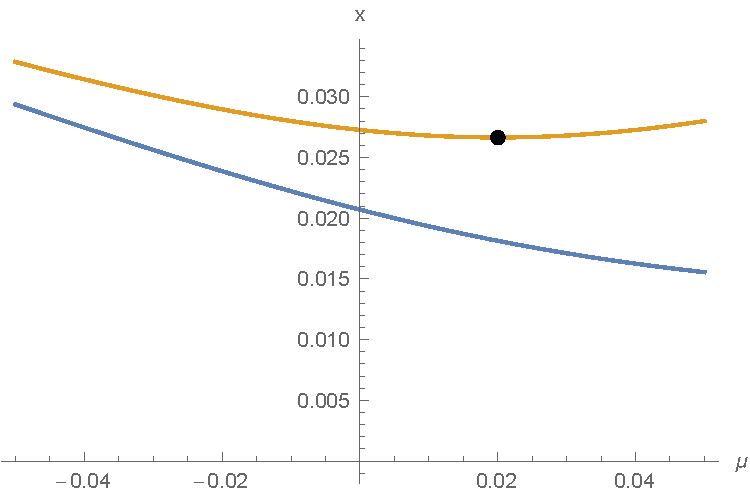
\includegraphics[width=0.45\textwidth]{Prob1_CapOpt/xopt_mu_sigma2.pdf}}
	\end{subfigmatrix}
	\caption{Behaviour of the threshold value with respect to the benchmark model (blue) and the capacity optimized model (orange), considering drift $\mu \in [-r, r]$ and corresponding stationary point $\sigma^2/2$ (black dot).}
	\label{fig:mu}
\end{figure}

%Regarding the drift parameter $\mu$ we obtained that the threshold values do not have a monotonic behaviour, either for smaller or bigger values of volatility. As showed in Figure \ref{fig:mu}, the smallest value of demand level necessary to invest is observed at the stationary point when $\mu=\sigma^2/2$.
As proved in Propositions \ref{1_prop1} and \ref{1_prop2}, the investment threshold does not have a monotonic behaviour w.r.t. $\mu$, as we show in Figure \ref{fig:mu}

For instance, when $\sigma=0.05$ (low volatility). By inspection of Figure  \ref{fig:mu} (a), we conclude that for $\mu<\frac{\sigma^2}{2}$, $x^*_B>x^*_C$, which leads to postponing the investment decision in the benchmark model. For larger values of $\mu$, the opposite is verified and thus, in the case the market is expected to grow, the investment decision occurs first without capacity optimization. This seems to be related with the fact that an increasing $\mu$ also impacts on $K_C^*$ - as can be seen on the leftmost side of Figure \ref{fig:k1}. So, a growing market leads also to an investment in larger capacity and thus higher values of demand are needed. Regarding $x^*_B$, its value doesn't seem to significantly decrease for a situation when the market is growing. This might whether be related with the low capacity chosen or with the small values of $\mu$ considered.

When the volatility is considerably higher, as in Figure \ref{fig:mu} (b) considering $\sigma=0.2$, we observe a clear dominance of $x^*_C$ with comparison with $x^*_B$, at least for the drift range considered.







\begin{figure}[!htb]
	\centering
	\subfigure[$\theta \in ( 1, 10)$ ]{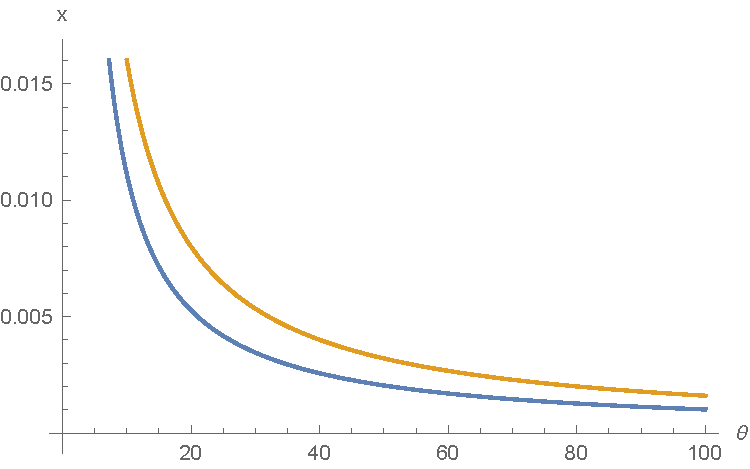
\includegraphics[width=0.45\textwidth]{Prob1_CapOpt/xopt_theta.pdf}}
	\caption{Behaviour of the threshold value with respect to the benchmark model (blue) and the capacity optimized model (orange) and decreasing parameter $\theta$.}
	\label{fig:td}
\end{figure}

Regarding the innovation breakthrough level, we obtain that the larger it is, the greater is the unitary price associated to the new product, so as market's expectation, and hence, the firm tends to anticipate its investment decision leading to smaller threshold values for both models, this is illustrated on Figure \ref{fig:td}.
%Regarding the innovation breakthrough we observe, on Figure \ref{fig:td}, that a higher $\theta$ implies a smaller demand threshold, regarding both models. This is in accordance to what was done in \cite{rita}, since as $\theta$ increases, the firm wills to invest in a product with much more advanced technology, that, taking into account our instantaneous profit function $\pi$ \eqref{prob1:pi}, will culminate in higher earnings, when fixing the demand value.



\subsection{Optimal Capacity Level}

Here we focus on the optimal capacity $K^*_C$ as it is presented in \eqref{prob1:K*}. We analyse how $K_C^*$ behaves with the different parameters.

\begin{prop}
	\label{1_prop3}
The optimal capacity level $K^*_C$ increases with $\mu$, $\sigma$ and $\theta$, decreases with $r$ and $\alpha$, and it is independent on $\delta$.
\end{prop}


\textbf{Proof:}
The relation between $K^*_C$ and $\theta$, $r$ or $\alpha$ comes immediately by observing $K^*_C$'s formula.

Now, regarding drift parameter we obtain that
 \begin{align*}
\frac{\partial K^*_C(\mu)}{\partial \mu}=
\frac{4 \theta \left(\sigma ^2 \left(\phi+1\right)-2 \mu \right)}{\alpha \phi \left(\sigma ^2 \left(\phi+3\right)-2 \mu \right)^2}>0.
\end{align*}
The numerator is positive since
\begin{align}
\label{cond2}
\sigma ^2 (\phi+1)=\sigma ^2 \left(\sqrt{\frac{4 \mu ^2}{\sigma ^4}-\frac{4 \mu }{\sigma ^2}+\frac{8 r}{\sigma ^2}+1}+1\right)-2 \mu>0 
& \Leftrightarrow
\frac{4 \mu ^2}{\sigma ^4}-\frac{4 \mu }{\sigma ^2}+\frac{8 r}{\sigma ^2}+1 > \left( \frac{2 \mu}{\sigma^2}-1 \right)^2=\frac{4 \mu ^2}{\sigma ^4}-\frac{4 \mu }{\sigma ^2}+1 \nonumber\\
& \Leftrightarrow
\frac{8 r}{\sigma ^2}>0 \nonumber
\end{align}
holds for $\forall r> 0$. As the denominator is clearly positive, the result is verified.

Regarding volatility parameter we obtain that
\begin{equation*}
    \frac{\partial K^*_C(\sigma)}{\partial \sigma}= 
\frac{8 \theta \left(2 \mu ^2-\mu  \sigma ^2 \left( \phi+1 \right)+2 r \sigma ^2 \right)}{\alpha \sigma  \phi  \left( \sigma ^2 \left( \phi+3 \right)-2 \mu \right)^2}>0.
\end{equation*}
%From the negativity of the numerator in \eqref{sol}, it follows that the denominator here expressed is positive, from which the result holds.
By similar arguments than the ones used in \eqref{1_xBs}, we conclude that the numerator is positive, thus leading to the result.

%From \eqref{demo} we obtain that the denominator is positive and from \eqref{condd1} and \eqref{cond2} that the denominator is positive for $\forall r\geq0$, from which the result holds.
\begin{flushright}
	$\square$
\end{flushright}

In order to illustrate the previous result and to have an idea about the type of growth of $K^*_C$ w.r.t. the parameters, we add some plots for the numerical values considered in the beginning of this section.

\begin{figure}[!htb]
	\begin{subfigmatrix}{3}
		\subfigure[$\mu \in ( -r,r )$ ]{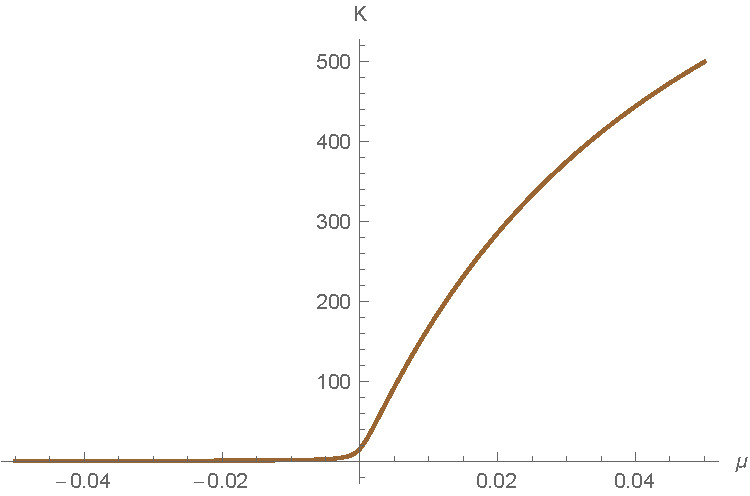
\includegraphics[width=0.32\textwidth]{Prob1_CapOpt/kopt_mu.pdf}}
		\subfigure[$\sigma \in (0,1)$]{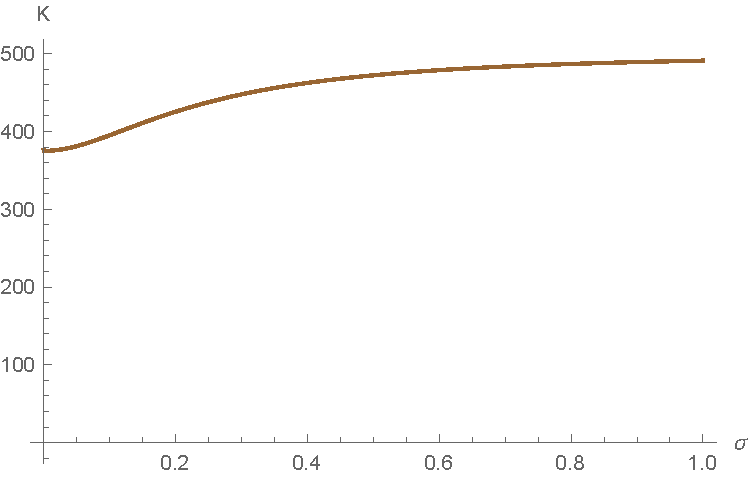
\includegraphics[width=0.32\textwidth]{Prob1_CapOpt/kopt_sigma.pdf}}
		\subfigure[$\theta \in (\alpha K^*_C,10)$]{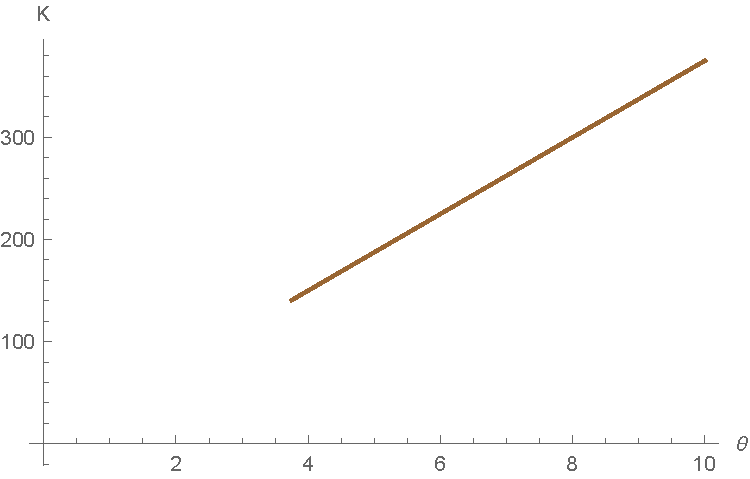
\includegraphics[width=0.32\textwidth]{Prob1_CapOpt/kopt_theta.pdf}}
	\end{subfigmatrix}
	\caption{Behaviour of the optimal capacity regarding the threshold value $x^*_C$ and increasing parameters $\mu$, $\sigma$ and $\theta$.}
	\label{fig:k1}
\end{figure}

On the leftmost side of Figure \ref{fig:k1} we study $K^*_C$ as a function of $\mu$. We note that the growth of $K^*_C$ is barely noticed on a decreasing market ($\mu<0$), but it turns to be logarithmic in a growing market ($\mu>0$). Mathematically, these behaviours are related with the fact that the denominator of $K^*_C$ decreases with $\mu$, in a weak rate for negative $\mu$ and in a significant rate for positive $\mu$. Financially, they are connected with the fact that in a growing market the demand is expected to be larger than in a decreasing market and hence, the capacity should be larger in order to be able to satisfy market needs.

On Figure \ref{fig:k1} (b), although in a weaker rate, the optimal capacity seems to increase with volatility.

As expected, on Figure \ref{fig:k1} (c) we observe that $K^*_C$ grows linearly with the chosen innovation level, being this fact related with the expected market response to a newer technology.
%Considering some numerical approximations, we observe, on Figure \ref{fig:k1}, that $K^*_C$ increases with drift, volatility and innovation level, as deduced before. Note that, regarding the drift parameter, the growth is barely noticeable for negative values of $\mu$, but then it turns to be logarithmic.
%This is related with the fact that the denominator of $K_C^*$ decreases with $\mu$. For $\mu<0$, the denominator increases in a weak rate, resulting in an almost constant value of $K^*_C$. However, when $\mu>0$, as it increases, the denominator decreases significantly, resulting in higher values of $K^*_C$.

%Regarding volatility $\sigma$, we obtain that the optimal capacity increases with it, however in a weaker rate.

%Regarding the innovation breakthrough $\theta$, $K^*_C$ shows to increase linearly with it.
%FINANCIAL INTERPRETATION? This seems to be related with the fact that for small drift values, the future expected demand value is smaller that for positive drift values. Recall that the demand process evolves accordingly to a GBM and its expected value at time $t$ is given by $\mathds{E} ^{X_0=x_0} [X_t]=x_0 e^{\mu t}$.

\begin{figure}[!htb]
	\begin{subfigmatrix}{2}
		\subfigure[$ r \in ( \mu, 1 )$]{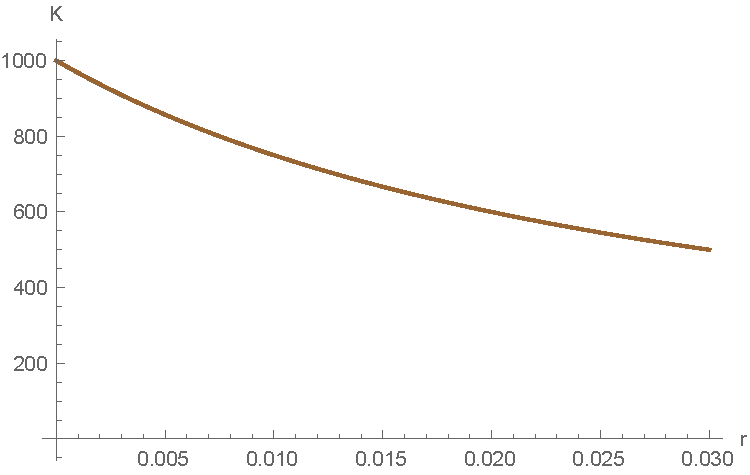
\includegraphics[width=0.45\textwidth]{Prob1_CapOpt/kopt_r.pdf}}
		\subfigure[$ \alpha \in (0,1)$]{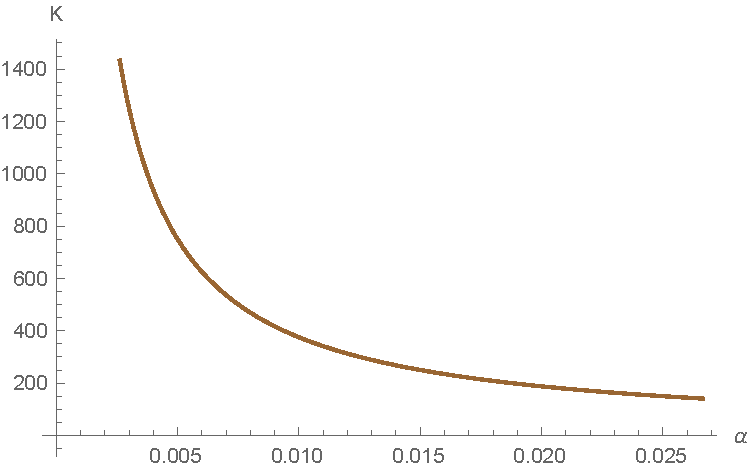
\includegraphics[width=0.45\textwidth]{Prob1_CapOpt/kopt_alpha.pdf}}
	\end{subfigmatrix}
	\caption{Behaviour of the optimal capacity regarding the threshold value $x^*_C$ and decreasing parameters $r$ and $\alpha$.}
	\label{fig:k2}
\end{figure}

Figure \ref{fig:k2} (a) shows the behaviour of $K^*_C$ w.r.t. the discount rate and, in (b), w.r.t. the sensibility parameter $\alpha$. Although in different rates, $K_C^*$ decreases with both parameters.
 
